\graphicspath{{background/fig/}}

\chapter{Background} \label{chap:background}
This chapter provides an overview of Automatic Speech Recognition (ASR), the general approach of ASR, and the common challenges of ASR.
We provide a detailed explanation of wav2vec 2.0, a framework for learning speech features.
We discuss how the connectionist temporal classification (CTC) algorithm is used to fine-tune speech features for ASR.
The chapter concludes with an explanation of why pre-training is infeasible for our study,
and a brief discussion of two already pre-trained wav2vec 2.0 models.

% ***************************************************
% SECTION 1
% ***************************************************
\section{The automatic speech recognition task}\label{sec:background}
Automatic speech recognition (ASR), also known as speech recognition, 
is the task of identifying the spoken words for a given speech recording and returning the text, or \emph{transcription}, of the spoken words.
For example, given a recording of a speaker\footnote{Speaker in this context refers to a person speaking, and not a loudspeaker.} saying the sentence ``The quick brown fox jumps over the lazy dog'',
the goal of ASR is to predict each character in the sentence and to make as few mistakes as possible.

The general approach for ASR involves two steps.
In the first step, we transform the speech recordings into a higher-dimensional feature representation called \emph{speech features}.
Then, in the second step we use supervised learning techniques to map speech features
to a sequence of characters that are merged into a sentence.

Computing speech features is useful because recording data is difficult to interpret. 
Recording data, or audio data, consists of a sequence of floating point numbers called \emph{samples}.
The sequence of samples represent amplitude measurements of the recorded sound wave. 
Note that sound is a continuous wave function, but a recording is a discretized version of the original sound (see Figure \ref{fig:wave}).
The issue is that mapping a sequence of samples to a sequence of characters is difficult.
Therefore, it is common in ASR and other speech-related tasks to transform audio data into speech features.
The traditional approach is to compute speech features by transforming the audio data from the amplitude-time domain 
to the frequency-time domain using the Fast Fourier Transform (FFT) algorithm \cite{cochran1967fast}, \cite{cooley1969fast}.

\begin{figure}
    \centering
    \captionsetup{justification=centering}
    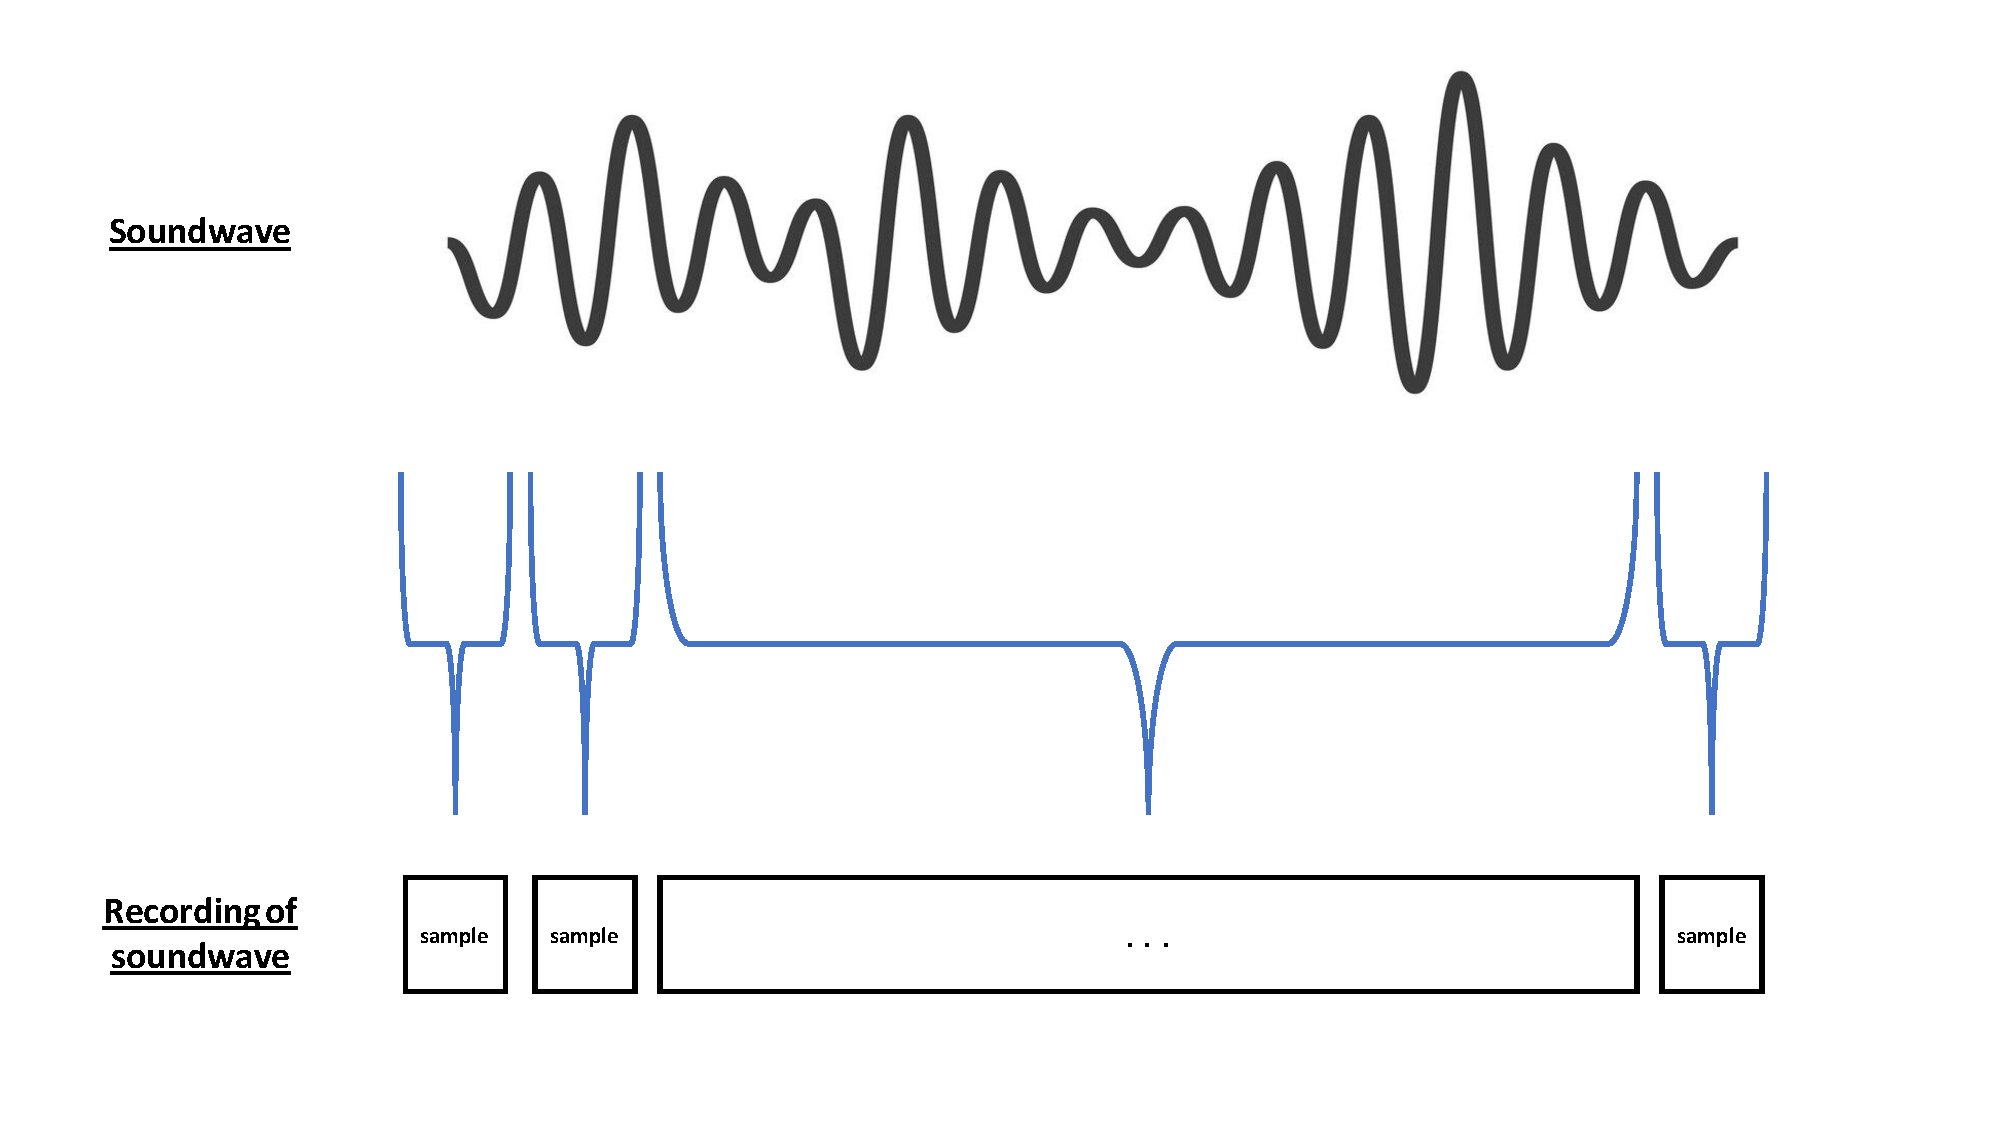
\includegraphics[width=0.8\textwidth]{wave.pdf}
    \caption{A diagram that explains what audio data represents. Note that this is an oversimplified explanation. The intent of the diagram is to explain why it is difficult to interpret raw audio data.}
    \label{fig:wave}
\end{figure}

In this study, we discuss an approach to obtain speech features using self-supervised learning.
Self-supervised learning is a machine learning paradigm in which unlabeled data is used for learning, similar to unsupervised learning.
Self-supervised learning differs from unsupervised learning in that it leverages the unlabeled data to create artificial labels, 
often through tasks designed to predict part of the input from other parts. 
For instance, in the context of speech features, a task of the model may be to predict the next sample of an audio sequence, 
using the previous samples as context.
This approach transforms the problem into a supervised problem without the need for explicit labels. 
Before explaining this approach, we discuss the importance of constructing good ASR datasets.

\subsection{Automatic speech recognition data}
The first step of creating an ASR model is to prepare audio datasets for training, evaluating, and testing the model.
A single dataset entry consists of a speech recording (of a spoken sentence) and the corresponding text of the spoken sentence.
The following paragraphs demonstrate why preparing each dataset
has a significant effect on the accuracy and generalization performance for ASR models.

\paragraph*{Exclusivity around partitioning data.}
The validation and test set should not contain recordings of voices that also appear in the training set.
This is to ensure that the model is not overfitting to the voices in the training set.

\paragraph*{The amount of training data.}
The training set should be as large as possible.
A larger training set often leads to better accuracy and generalization performance for ASR models.
A small dataset with few unique voices may lead to overfitting to the voices in the dataset.

\paragraph*{Voice diversity.}
The training set should contain a diverse set of speakers.
The accent of a speaker, which depends on the gender, age, and ethnicity of the speaker, 
may influence the generalization ability of ASR models. 
Generally, male voices have a lower pitch than female voices, and adults have a lower pitch than children.

\paragraph*{The difference between read and conversational speech.}
The training set should contain both read speech and conversational speech.
Speakers tend to speak more clearly when reading text from a transcript, in comparison to the speech of a conversation.
Recent ASR models obtain very low error rates for recordings of read speech \cite{jurafskyspeech}.
However, ASR for recordings of conversational speech is still a major challenge \cite{jurafskyspeech}.
% \paragraph*{The audio quality of recordings.}
% The training set should contain both low quality and high quality recordings.
% The position of the microphone,
% the quality of the microphone,
% the number of microphones available, 
% and the presence of background noise contribute towards the audio quality of recordings.
\\
\\
In the following section, we discuss wav2vec 2.0, which is the speech feature extraction technique used in this study.

% ***************************************************
% SECTION 2
% ***************************************************
\section{wav2vec 2.0}
wav2vec 2.0 provides a framework for learning speech features using unlabeled\footnote{Unlabeled audio data simply refers to recordings without transcription text (labels).} audio data.
wav2vec 2.0 can be applied to a variety of speech-related tasks such as ASR, automatic speech translation (AST),
and speech classification.
It proves to be particularly useful in cases where a lot of unlabeled data is available, but not much labeled data.
For ASR, the authors show that using just ten minutes of labeled data and pre-training
on 53k hours of unlabeled data achieves $4.8$/$8.2$ WER (\ref{subsec:wer}) on the clean/other test sets of the Librispeech~\cite{panayotov2015librispeech}.

The general two-step approach for using wav2vec 2.0 for any speech-related task is the following.
In the first step the wav2vec 2.0 model is trained (or ``pre-trained'') using unlabeled data, which
gives you a model that transforms audio data into speech features.
In the second step the model is fine-tuned on a downstream task using labeled data. 
Fine-tuning wav2vec 2.0 (\ref{subsec:finetune}) for ASR involves replacing the head of the 
pre-trained model with an appropriate loss function such as CTC (\ref{sec:ctc}).

\begin{figure}
    \centering
    \captionsetup{justification=centering}
    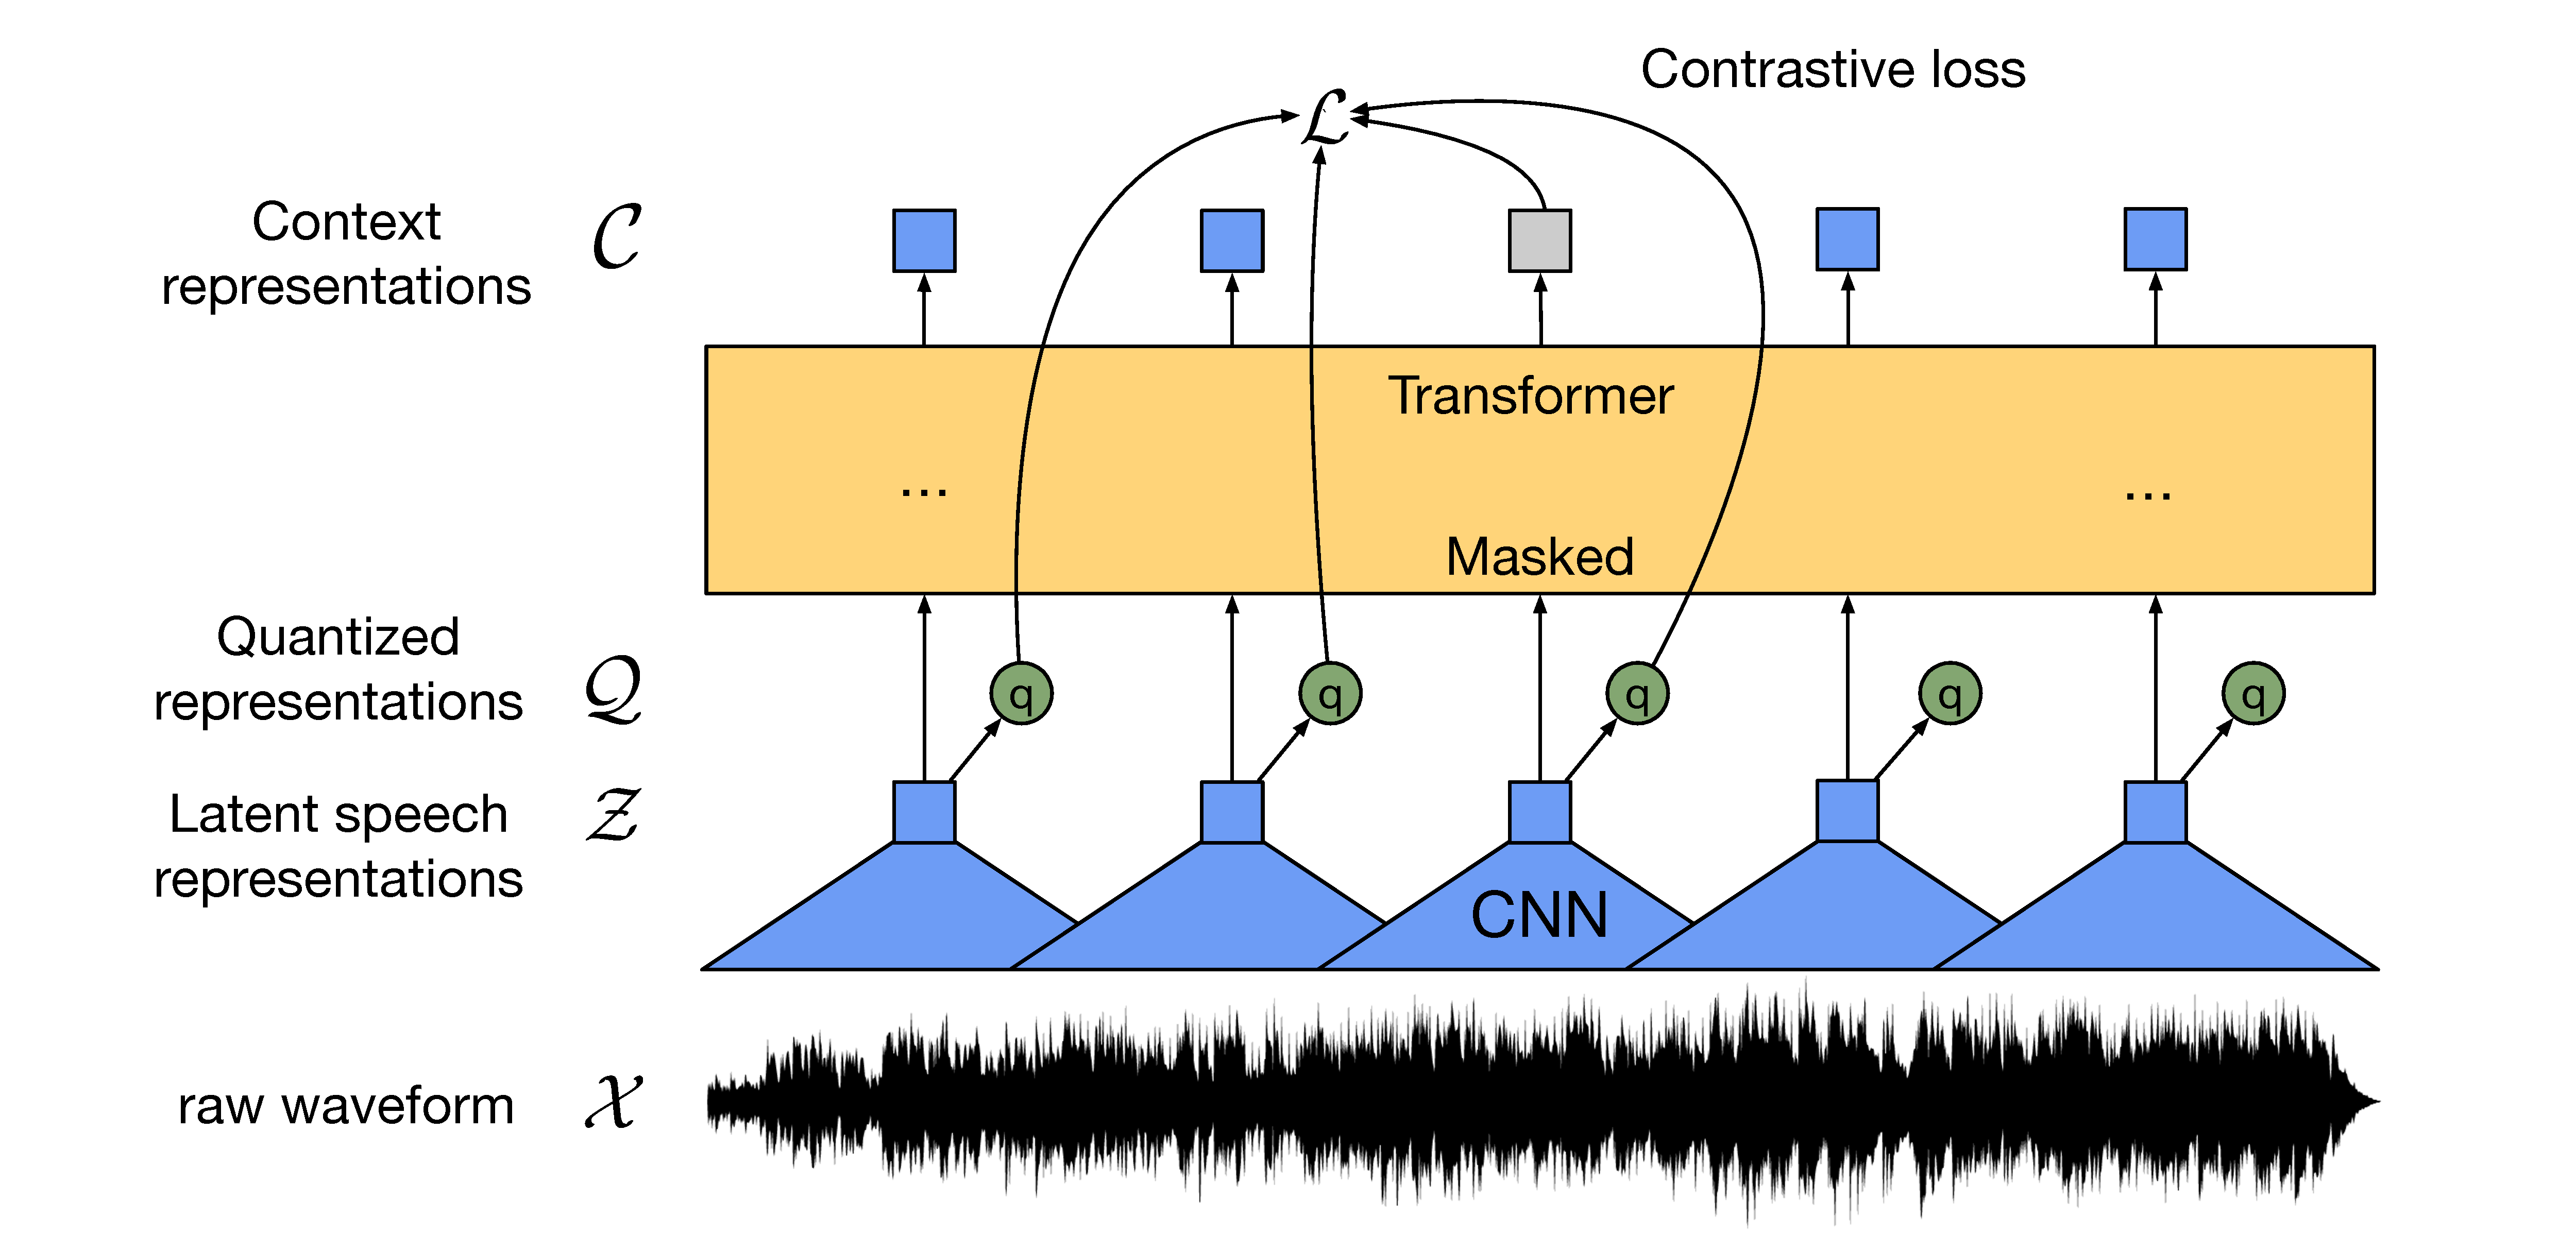
\includegraphics[width=\textwidth]{wav2vec2architecture.pdf}
    \caption{A visualization of the network architecture of wav2vec 2.0 \cite{baevski2020wav2vec}.}
    \label{fig:wav2vec2_architecture}
\end{figure}

The wav2vec 2.0 architecture is described by the network diagram in Figure~\ref{fig:wav2vec2_architecture}.
There are three important components of the architecture:
the feature encoder, the quantization module, and the context network.
The objective of wav2vec 2.0 becomes clear only after understanding each of the three
components. Therefore, we explain how to pre-train wav2vec 2.0 after explaining
the three components in detail.

\subsection{Feature encoder}
The feature encoder maps audio data to latent speech representations: $f: \mathcal{X} \rightarrow \mathcal{Z}$.
In other words, the feature encoder $f$ maps a sequence of audio samples $\mathbf{x}^{(1)}, \dots \mathbf{x}^{(N)}$ into a sequence of latent feature vectors $\mathbf{z}^{(1)}, \dots, \mathbf{z}^{(t)}$.

The audio data is scaled to have zero mean and unit variance before being fed into the feature encoder. 
The feature encoder consists of seven convolutional blocks, where each convolutional block contains a temporal convolutional layer,
layer normalization \cite{ba2016layer}, and the GELU \cite{hendrycks2016gaussian} activation function.

Each temporal convolutional layer contains $512$ channels, the strides of the seven temporal convolutional layers are $(5,2,2,2,2,2,2)$, and the kernel widths are $(10,3,3,3,3,2,2)$.
This results in each $\mathbf{z}^{(t)}$ representing $25$ ms of audio (or $400$ input samples), strided by about $20$ ms.
Layer normalization scales the logits after each convolutional layer to have zero mean and unit variance, which has been shown to increase the chances of earlier convergence.
GELU is an activation function recently used for several NLP-related tasks.


\subsection{Quantization module}
The quantization module maps the latent feature vectors into discrete speech units: $h: \mathcal{Z} \rightarrow \mathcal{Q}$.
Unlike written language, which can be discretized into tokens such as characters or sub-words, speech does not have natural sub-units \cite{bgn2021illustrated}.
This is because speech is a sound wave, which is a continuous function of time.
The quantization module is a method in which discrete speech units are automatically learned using product quantization.

To perform product quantization, the quantization module uses $G$ \emph{codebooks}, where each codebook contains $V$ \emph{codebook entries} $\mathbf{e}_{1}, \dots, \mathbf{e}_{V}$.
The following steps describe the process of automatically assigning a discrete speech unit to each latent feature vector $\mathbf{z}^{(t)}$:
\begin{enumerate}
    \item Transform $\mathbf{z}^{(t)}$ into $\mathbf{l}^{(t)} \in \mathbb{R}^{G \times V}$ using a linear transformation (feed-forward neural network).
    \item Choose one codebook entry $\mathbf{e}_g$ for each codebook $g = 1, \dots, G$, based on the values of $\mathbf{l}^{(t)}$.
    \item Concatenate the codebook entries $\mathbf{e}_1, \dots, \mathbf{e}_G$.
    \item Transform the resulting vector into $\mathbf{q}^{(t)} \in \mathbb{R}^{f}$ using another linear transformation (feed-forward neural network).
\end{enumerate}
The two linear transformations are feed-forward neural networks $\text{FF}_1: \mathbb{R}^{f} \rightarrow \mathbb{R}^{G \times V}$ and $\text{FF}_2: \mathbb{R}^{d} \rightarrow \mathbb{R}^{f}$.
In the second step above, the codebook entry $\mathbf{e}_g$ is chosen as the one with the argmax of the logits $\mathbf{l}$. Choosing the codebook entries in this way is non-differentiable.
Fortunately, we can use the Gumbel softmax to choose codebook entries in a fully differentiable way. 
$\mathbf{e}_g$ is chosen as the entry that maximizes
\begin{equation}
    p_{g, v} = \dfrac{\exp{\left(\mathbf{l}^{(t)}_{g, v} + n_v\right)}/\tau}{\sum\limits_{k=1}^{V} \exp{\left(\mathbf{l}^{(t)}_{g, k} + n_k\right)}/\tau},
\end{equation}
where $\tau$ is a non-negative temperature, $n = -\log{(-\log{(u)})}$, and $u$ are uniform samples from $\mathcal{U}(0, 1)$.
During the forward pass the codeword $i$ is chosen by $i = \text{argmax}_j p_{g,j}$, and during the backward pass the true gradient of the Gumbel softmax outputs is used.

\subsection{Context network}
% Explain what it is and its purpose
The context network maps the latent feature vectors into contextualized representations: $g: \mathcal{Z} \rightarrow \mathcal{C}$.
The main component of the context network is a Transformer encoder \cite{transformer}.
Due to the popularity of Transformers, we omit the details of the Transformer architecture.
However, we recommend illustrated guides such as \cite{alammar2018illustrated} for more information about the Transformer architecture.

% Explain architecture further
The following steps describe how the latent feature vectors are processed before being fed into the Transformer encoder.
\begin{enumerate}
    \item The latent feature vectors are fed into a \emph{feature projection layer} to match the model dimension of the context network.
    \item Positional embedding vectors are added to the inputs using \emph{relative positional encoding} \cite{shaw2018relative} instead of absolute positional encoding.
    The relative positional encoding is implemented using grouped convolution \cite{AlexNet}.
    \item Inputs are fed into the GELU activation function, followed by layer normalization.
\end{enumerate}

The output after processing the latent feature vectorsaccording to the steps above are fed into the Transformer encoder, which results in
a sequence of contextualized representations $\mathbf{c}^{(1)}, \dots \mathbf{c}^{(T)}$.
The details for the Transformer encoder of the \textsc{LARGE} version of wav2vec 2.0 are:
\begin{itemize}
    \item Number of Transformer blocks: $B = 24$.
    \item Model dimension: $H_m = 1024$.
    \item Inner dimension: $H_{ff} = 4096$.
    \item Number of attention heads: $A = 16$.
\end{itemize}

\subsection{Pre-training with wav2vec 2.0}
Here we discuss how the three components are used to perform pre-training with wav2vec 2.0.
The main objective of pre-training is a contrastive task, which involves masking a proportion of the output of the feature encoder ($\mathbf{z}^{(1)}, \dots, \mathbf{z}^{(t)}$).

A proportion of the latent feature vectors are masked and replaced by a shared feature vector $\mathbf{z}_{\text{M}}$, before being fed into the context network.
Note, that the inputs to the quantization module are not masked.
A proportion $p$ of starting indices in $\{1, \dots, t\}$ are randomly sampled. 
Then, for each starting index $i$, consecutive $M$ time steps are masked (where spans may overlap).

The dimensionality of the output of the context network ($\mathbf{c}^{(1)}, \dots \mathbf{c}^{(T)}$) matches the dimensionality of the 
output of the quantization module ($\mathbf{q}^{(1)}, \dots \mathbf{q}^{(T)}$).
The contrastive task involves predicting the corresponding quantized target $\mathbf{q}^{(t)}$ for a context vector $\mathbf{c}^{(t)}$.
Additionaly, $100$ negative distractors are uniformly sampled for each masked position.
The model is encouraged to minimize the distance (cosine similarity) between $\mathbf{q}^{(t)}$ and $\mathbf{c}^{(t)}$, and to maximize the distance between $\mathbf{q}^{(t)}$ and the negative distractors.
A detailed explanation of the training objective follows below.

\paragraph*{Training objective.} There are two objectives (loss functions) that wav2vec 2.0 optimizes simultaneously.
The first loss function is the contrastive loss $\mathcal{L}_m$ which encourages the model to
identify the true quantized representation for a masked time step within a set of distractors. 
The second loss function is the diversity loss $\mathcal{L}_d$ which encourages the model 
to equally use the codebook entries from the quantization module.
The full training objective is given by $\mathcal{L} = \mathcal{L}_m + \alpha \mathcal{L}_d$, where $\alpha$ is a tuned hyperparameter.

\paragraph*{Contrastive loss.}
The contrastive loss is responsible for training the model to predict the correct quantized 
representation $\mathbf{q}_t$ from a set of candidate representations $\mathbf{\tilde{q}} \in \mathcal{Q}_t$. 
The set $\mathcal{Q}_t$ includes the target $\mathbf{q}_t$ and $K$ distractors sampled uniformly from other masked time steps. 
The contrastive loss is given by
\begin{equation}
    \mathcal{L}_m = -\log \dfrac{\exp(\text{sim}(\mathbf{c_t}, \mathbf{q_t}) \/ \kappa)}{\sum_{\mathbf{\tilde{q}} \sim \mathcal{Q}_t} \exp(\text{sim}(\mathbf{c_t}, \mathbf{\tilde{q}}) \/ \kappa)},
\end{equation}
where $\kappa$ represents a constant temperature, and $\text{sim}(a, b)$ denotes the cosine similarity between 
context representation $c_t$ and quantized representations $q$. 
This loss encourages the model to assign high similarity to the true 
positive target and penalize high similarity with negative distractors.

\paragraph*{Diversity loss.}
The diversity loss is a regularization technique aimed at promoting the equal use of codebook entries. 
It is based on entropy and is calculated as:
\begin{equation}
    \mathcal{L}_d = \dfrac{1}{GV}\sum_{g=1}^{G} -H(\bar{p}_{g}) = -\dfrac{1}{GV}\sum_{g=1}^{G} \sum_{v=1}^{V} \bar{p}_{g,v} \log \bar{p}_{g,v}.
\end{equation}
This loss maximizes the entropy of the softmax distribution $\bar{p}_{g,v}$ over codebook entries, encouraging the model to utilize all code words equally.

\subsection{Fine-tuning wav2vec 2.0 for automatic speech recognition}\label{subsec:finetune}
To fine-tune a pre-trained wav2vec 2.0 model for ASR, it is required to prepare a labeled dataset.
Typically, the head of the model is replaced with a linear layer that has an equal number of output neurons as the size of the vocabulary\footnote{The vocabulary refers to the set of unique characters contained in the transcriptions (labels) of the dataset.} of the labeled dataset.
The model is optimized using a supervised learning algorithm called connectionist temporal classification.

% ***************************************************
% SECTION 3
% ***************************************************
% Output text OR sentence?
\section{Connectionist temporal classification}\label{sec:ctc}
Connectionist temporal classification (CTC) \cite{graves2006connectionist} is an algorithm 
developed to map a sequence of speech features to a sequence of characters.
Our explanation of CTC is heavily based on the speech recognition and text-to-speech chapter in \cite{jurafskyspeech}.
We recommend readers to use Figure~\ref{ctc} as a visual aid for our explanation.

\begin{figure}
    \centering
    \captionsetup{justification=centering}
    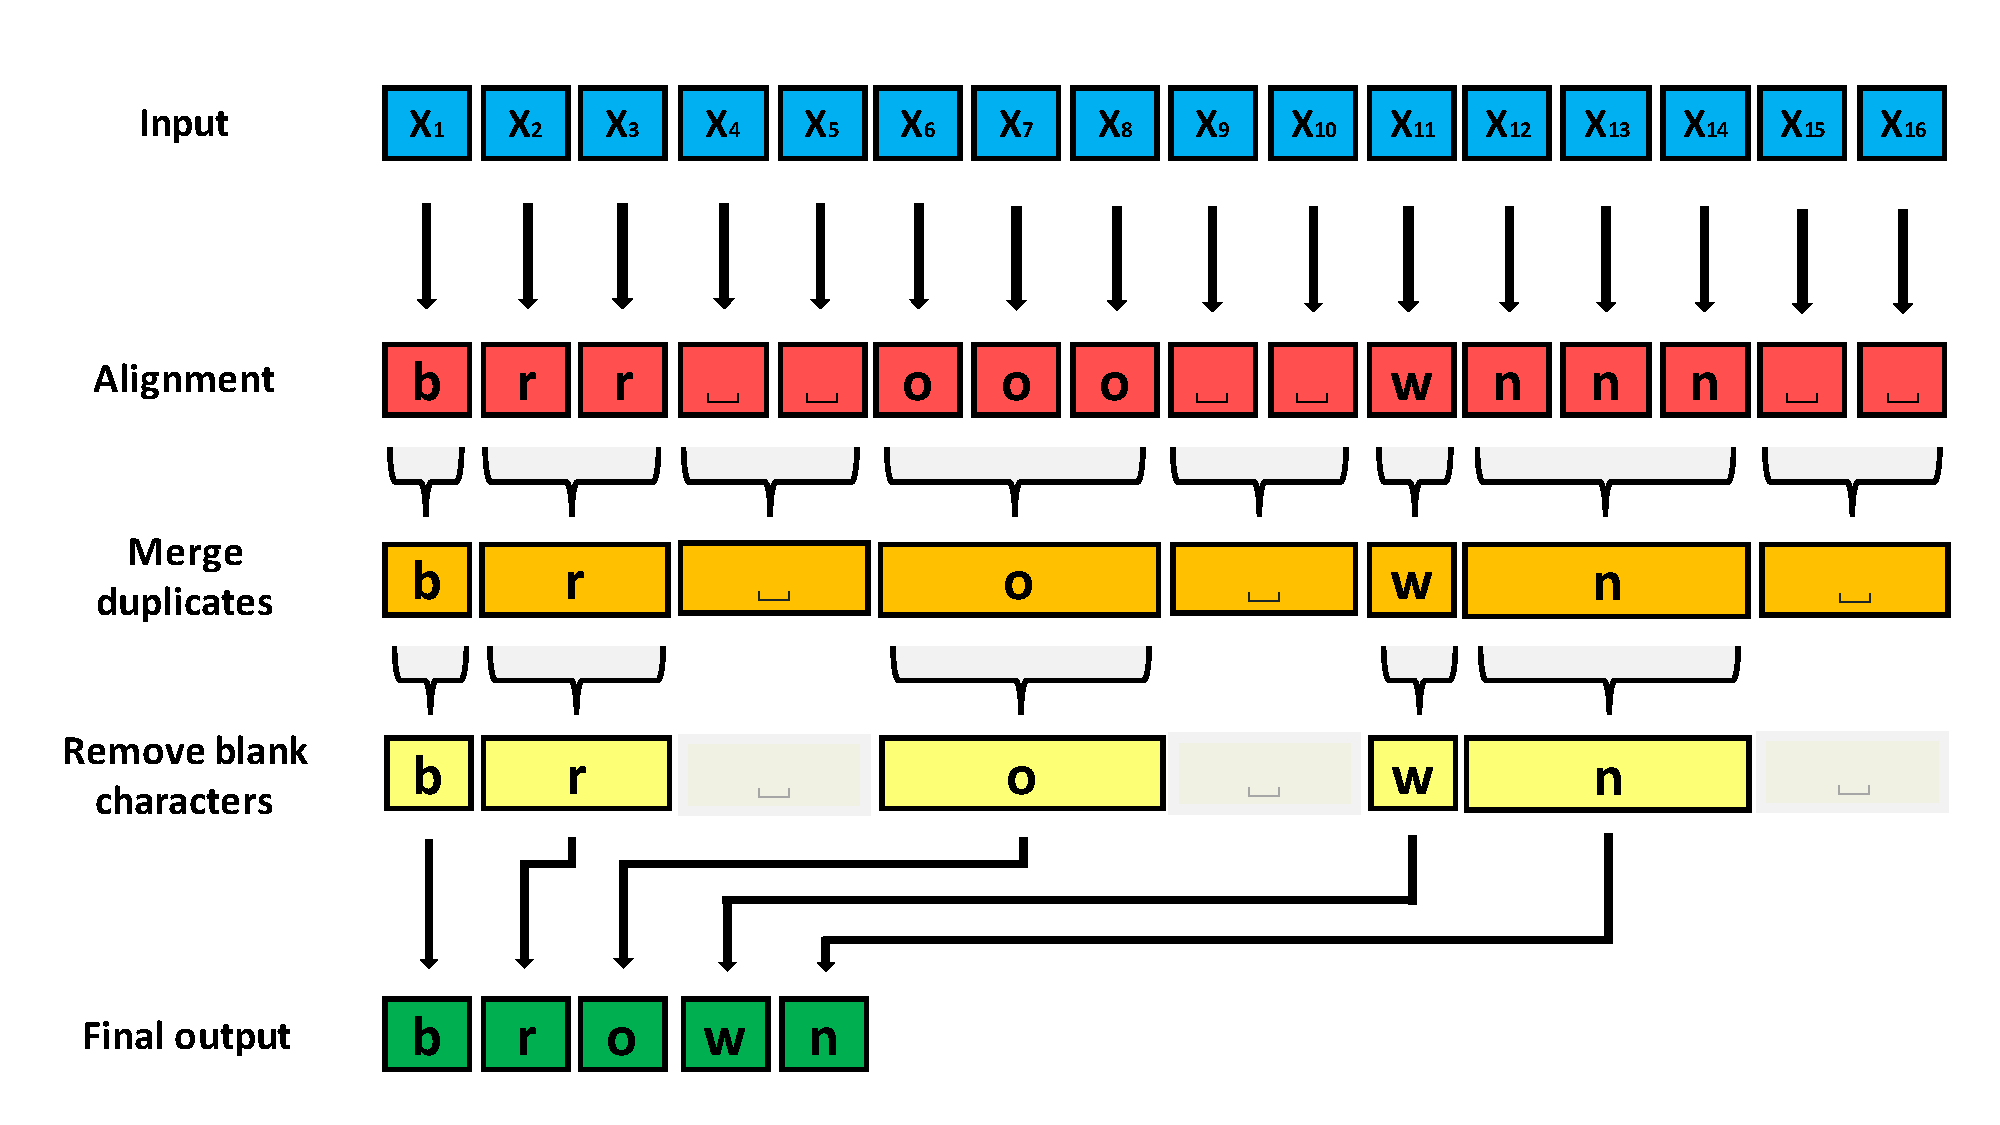
\includegraphics[width=0.8\textwidth]{ctc.pdf}
    \caption{A diagram that describes the alignment procedure of CTC \cite{jurafskyspeech}.}
    \label{ctc}
\end{figure}

Given a sequence of speech features, CTC maps each speech feature vector to a single character, which results in a sequence of characters known as an \emph{alignment}. 
Then, a \emph{collapsing function} is used to merge consecutive duplicate characters in the alignment.
The authors of CTC propose the use of a special character called a \emph{blank}, which is represented by ``\textvisiblespace''.
The blank character accounts for words that contain consecutive duplicate characters (such as the word ``dinner'', which contains two consecutive ``n'' characters).
With the addition of the blank character, the collapsing function is responsible for merging consecutive duplicate characters and removing all instances of blank characters.
Following the notation of \cite{jurafskyspeech}, we define the collapsing function as a mapping $B: A \rightarrow Y$ for an alignment $A$ and output text $Y$.
Notice that $B$ is many-to-one, since many different alignments can map to the same output text (see Figure~\ref{dinner}).

\begin{figure}
    \centering
    \captionsetup{justification=centering}
    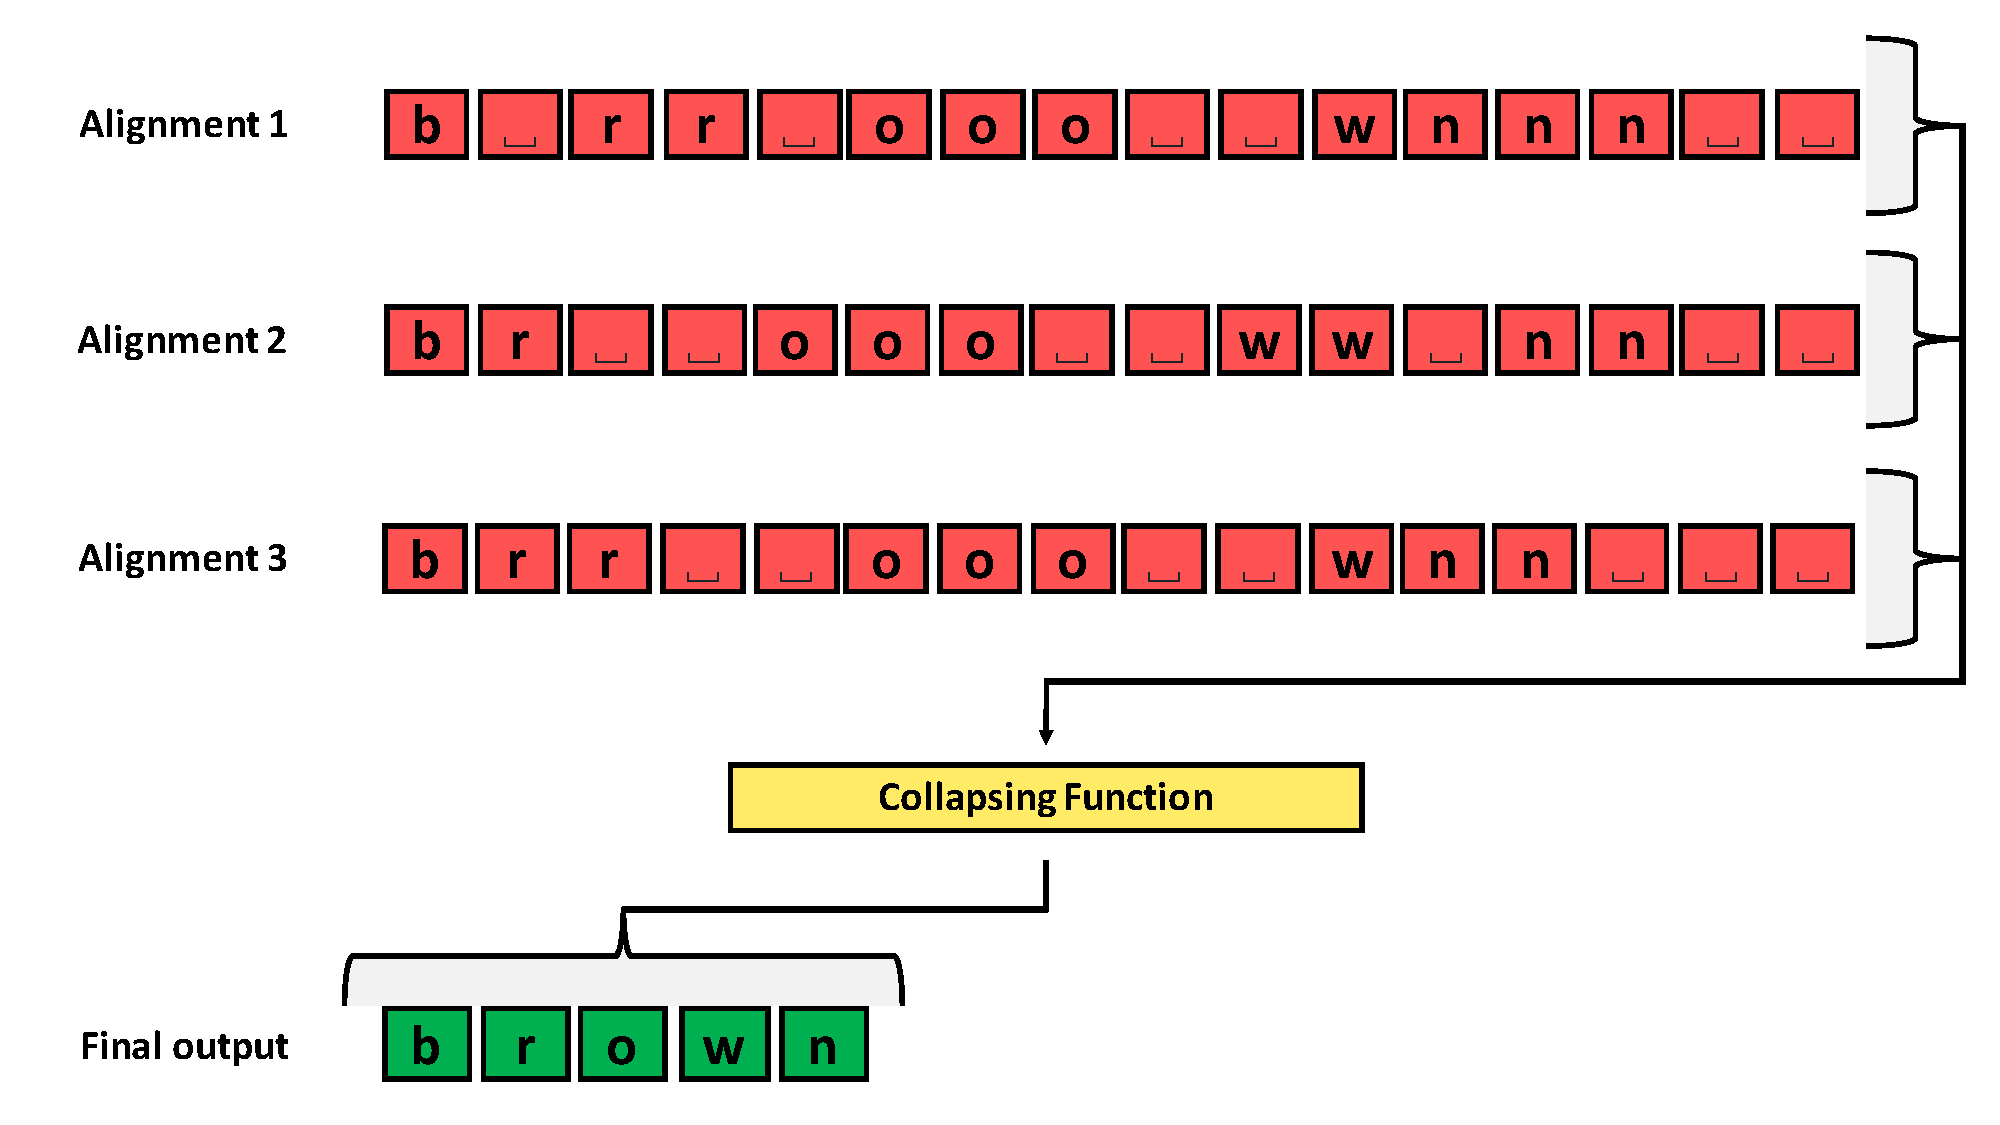
\includegraphics[width=0.75\textwidth]{3alignments.pdf}
    \caption{Three different alignments that produce the same output text when using the CTC collapsing function \cite{jurafskyspeech}.}
    \label{dinner}
\end{figure}

In \cite{jurafskyspeech}, the set of all alignments that map to the same output text $Y$ is denoted as $B^{-1}(Y)$, 
where $B^{-1}$ is the inverse of the collapsing function.
This notation is useful for our explanation of CTC inference and training.

\subsection{Connectionist temporal classification inference}
Here we discuss how CTC models the probability of the output text $Y$ 
for a sequence of speech features $X = \{x^{(1)}, \dots, x^{(T)}\}$, 
denoted by $P_{\text{CTC}}(Y|X)$.
The conditional probability above can be expressed as the summation over the probabilities
of all possible alignments that produce the output text $Y$. 
Hence, we obtain the expression: 
\begin{equation}
    P_{\text{CTC}}(Y|X) = \sum\limits_{A \in B^{-1}(Y)} P(A|X).
\end{equation}

We still need an expression for $P(A|X)$.
To compute $P(A|X)$, CTC makes a strong conditional independence assumption. 
It assumes that each alignment character $a^{(t)} \in \{a^{(1)}, \dots, a^{(T)}\}$ 
is computed independently of all the other alignment characters.
Hence, we obtain the expression:
\begin{equation}
    P(A|X) = \prod\limits_{t=1}^{T} p(a^{(t)} | x^{(t)}).
\end{equation}

Now we can find the best possible alignment for a given $X$, by simply choosing the most probable character at each time step.
We compute each alignment character $\{a^{(1)}, \dots, a^{(T)}\}$, apply the collapsing function, and obtain the output text $Y$.
However, there is an issue with the greedy approach described above. 
The issue is that the most probable output text $\hat{Y}$ may not correspond
with the most probable alignment sequence $\{\hat{a}^{(1)}, \dots, \hat{a}^{(T)}\}$.
The reason for this is that there are many possible alignments that lead to the same
output text. Therefore, the most probable output text $\hat{Y}$, for a given $X$, corresponds to the maximum summation over the probabilities of all its
possible alignments:

\begin{align}
    \hat{Y} = \text{argmax}_Y P_{\text{CTC}}(Y|X) &= \text{argmax}_Y \left(\sum\limits_{A \in B^{-1}(Y)} P(A|X)\right) \\
                                                               &= \text{argmax}_Y \left(\sum\limits_{A \in B^{-1}(Y)} \prod\limits_{t=1}^{T} p(a^{(t)} | x^{(t)})\right).
\end{align}

There are many possible alignments, and summing over all the possible alignments is expensive and infeasible.
We can use dynamic programming to approximate this sum, by using a modified version of Viterbi beam search \cite{hannun2017sequence}. 
The beam search returns a user-specified number of potential output texts, 
and a loss function is used to score each output text.
The text with the best score is chosen as the final prediction.

\subsection{Connectionist temporal classification training}
The CTC training objective function is the negative log-likelihood.
Formally, the loss for a dataset $D$ is equal to the summation of the negative log-likelihoods 
of the correct output $Y$ for each corresponding input $X$:
\begin{align}
    L_{\text{CTC}} &= \sum_{(X,Y) \in D} -\log P_{\text{CTC}}(Y|X) \\
                    &= \sum_{(X,Y) \in D} -\log \left( \sum_{A \in B^{-1}(Y)} \prod_{t=1}^{T} p(a^{(t)} | x^{(t)}) \right).
\end{align}

Once again, we cannot compute a summation over all the possible alignments.
The summation is efficiently computed using a variant of the \emph{forward-backward algorithm}.
A detailed explanation of the forward-backward algorithm used for training CTC is given in \cite{hannun2017sequence}.

\subsection{Improving connectionist temporal classification with a language model.} \label{subsec:lm-boost}
Because of the strong conditional independence assumption mentioned earlier,
CTC does not implicitly learn a language model over the data.
Therefore, the CTC algorithm commonly predicts sentences that contain obvious spelling mistakes.
We can mitigate this issue by using a seperately trained language model (LM).
This is done by adding an additional term in the CTC loss function with interpolation weights:

\begin{equation}
    \text{score}_{\text{CTC}}(Y|X) = \log\left(P_{\text{CTC}}(Y|X)\right) + \lambda_1 \log\left(P_{\text{LM}}(Y)\right) + \lambda_2 L(Y).
\end{equation}
\hl{TODO}: briefly unpack what $P_{\text{LM}}(Y)$ is, and how it would be constructed

We have now discussed how to create an ASR model that is pre-trained using wav2vec 2.0 and fine-tuned using CTC. 
However, in the following section we discuss an issue with this approach for our particular study.



% ***************************************************
% SECTION 4
% ***************************************************
\section{The difficulty of pre-training using wav2vec 2.0}
Pre-training with wav2vec 2.0 using unlabeled data is infeasible for our study because:
\begin{enumerate}
    \item Pre-training with wav2vec 2.0 is known to be quite unstable (see ``NOTE 1'' of \cite{vonplaten2021pretraining}).
    \item Performing one experiment (run) of the large-scale wav2vec 2.0 model, using 8 GPU V100s (16 GB RAM each), takes 7 days to finish \cite{vonplaten2021pretraining}.
\end{enumerate}
At the time of conducting this study, we did not have access to the computational resources required to perform pre-training experiments.
Therefore, our study focuses on fine-tuning already pre-trained wav2vec 2.0 models, rather than performing pre-training and then fine-tuning.
In this section, we discuss the pre-trained models used in this study: \href{https://huggingface.co/facebook/wav2vec2-large}{Wav2Vec2-Large} and XLS-R.
Wav2Vec2-Large \cite{baevski2020wav2vec} is a base-sized wav2vec 2.0 model pre-trained on $960$ hours of English speech recordings.

\subsection{XLS-R}
XLS-R \cite{babu2021xls} is a large-scale wav2vec 2.0 model trained on $128$ different languages to learn \emph{cross-lingual} speech representations.
XLS-R attempts to build better representations for low-resource languages by leveraging cross-lingual transfer from high-resource languages such as English.

The model is trained using batches that contain samples from multiple languages $L$. 
Batches are sampled from a probability distribution $p_l \sim \left(\dfrac{n_l}{N}\right)^{a}$ where:
\begin{itemize}
    \item $l \in \{1, \dots, L\}$ represents each language.
    \item $N$ is the number of hours of all the unlabeled data and $n_l$ is the number of hours of unlabeled data for the language $l$.
    \item $\alpha$ controls how much data is chosen from the high-resource and low-resource languages.
\end{itemize}
\hl{TODO}: Give an intution for why this strategy is used.

The total number of hours of all the unlabeled data combined is about 436k hours. The authors use data from 24 high-resource languages, 17 mid-resource languages, and 88 low-resource languages.
The high-resource languages contain more than 1k hours of data each, the mid-resource languages contain more than 100 hours (but less than 1k hours)
of data each, and the low-resource languages contain less than 100 hours of data each.

XLS-R is evaluated on a wide range of downstream tasks: ASR, AST, and speech classification which includes language identification (LID) and speaker identification (SID).
XLS-R achieves better evaluation results than the previous state-of-the-art for several benchmark datasets for every downstream task,
which demonstrates the generalization ability of XLS-R.